%%% PostgreSQL Conference Europe 2013, Dublin, Oct 29, 2013
%%%
%%% What extensions are available? Where do you get them from? How to write
%%% Extensions, including portability, multi-version compatibility and
%%% controls. Includes discussion of new 9.3 feature background workers.

\documentclass{beamer}

\usepackage[utf8]{inputenc}

\usepackage{minted}

\usepackage{beamerthemesplit}
\usetheme{Boadilla}
%\setbeamertemplate{itemize items}{\checkmark}
\setbeamertemplate{itemize items}[circle]
\beamertemplatetransparentcovered

\usepackage{multicol}

\title{Writing \& using Postgres Extensions}
\subtitle{Postgre Open, Chicago, 2014}
\author{Dimitri Fontaine \texttt{dimitri@2ndQuadrant.fr}}
\date{Sept 17, 2014}
\logo{
\includegraphics[height=0.4cm]{2ndQuadrant-cross.png}}

\begin{document}

\frame{\titlepage}

\begin{frame}[fragile]
  \frametitle{Dimitri Fontaine}

  \begin{center}
    \textbf{2ndQuadrant France}
    \linebreak
    PostgreSQL Major Contributor
  \end{center}
  \vfill

\begin{columns}[c]
\column{.75\textwidth} 

  \begin{itemize}
   \item \texttt{pgloader}, \texttt{prefix}, \texttt{skytools}, …
   \item \texttt{apt.postgresql.org}
   \item \texttt{\textbf{CREATE EXTENSION}}
   \item \texttt{\textbf{CREATE EVENT TRIGGER}}
   \item MySQL migration tool, new \texttt{pgloader} version
  \end{itemize}  

\column{.25\textwidth}
\begin{center}
  
\includegraphics[height=7em]{2ndQuadrant-cross.png}
\end{center}
\end{columns}
\end{frame}

\begin{frame}[fragile]
  \frametitle{Writing \& using Postgres Extensions}

  \center{Agenda}
  \vfill

\begin{columns}
\column{.7\textwidth}

  \begin{itemize}
  \item How PostgreSQL extensibility works
  \item Things you can do with a PostgreSQL Extension
  \item The PostgreSQL indexing Framework
  \item \textbf{How to solve some practical use cases with existing extensions}
  \item Developping a new extension
  \end{itemize}

\column{.3\textwidth}
\begin{center}
  
\includegraphics[height=6em]{agenda.jpg}
\end{center}
\end{columns}
\end{frame}

\section{PostgreSQL Extensibility}

\begin{frame}[fragile]
  \frametitle{PostgreSQL Extensibility}

  \center{PostgreSQL is \textit{highly} \textbf{extensible}}
  \vfill

\begin{center}
  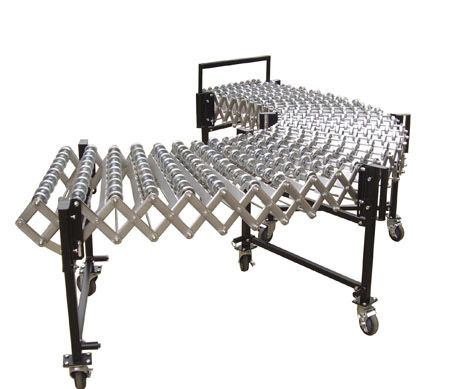
\includegraphics[height=15em]{extensible.jpg}
\end{center}
\end{frame}

\begin{frame}[fragile]
  \frametitle{PostgreSQL Extensibility}

\begin{minted}{postgresql}
select col1, col2 from table where col1 = 'something';
\end{minted}
\end{frame}

\begin{frame}[fragile]
  \frametitle{PostgreSQL Extensibility}

\begin{minted}{postgresql}
  SELECT col
    FROM table
   WHERE stamped > date 'today' - interval '1 day';
\end{minted}
\end{frame}

\begin{frame}[fragile]
  \frametitle{PostgreSQL Extensibility}

\begin{columns}
\column{.7\textwidth}
\begin{minted}{postgresql}
select iprange, locid
  from geolite.blocks
 where iprange >>= '91.121.37.122';


          iprange          | locid 
---------------------------+-------
 91.121.0.0-91.121.159.255 |    75
(1 row)

Time: 1.220 ms
\end{minted}
\end{columns}
\end{frame}

\begin{frame}[fragile]
  \frametitle{PostgreSQL Extensibility: Operator Classes}

  \center{SQL Operators are all dynamic and found in the catalogs}
  \vfill

\begin{columns}
\column{.7\textwidth}
\begin{minted}{postgresql}
select amopopr::regoperator
  from pg_opclass c
  join pg_am am
    on am.oid = c.opcmethod
  join pg_amop amop
    on amop.amopfamily = c.opcfamily
 where opcintype = 'ip4r'::regtype
   and am.amname = 'gist';
\end{minted}  
\column{.3\textwidth}
\begin{minted}{postgresql}
    amopopr     
----------------
 >>=(ip4r,ip4r)
 <<=(ip4r,ip4r)
 >>(ip4r,ip4r)
 <<(ip4r,ip4r)
 &&(ip4r,ip4r)
 =(ip4r,ip4r)
(6 rows)
\end{minted}
\end{columns}
\end{frame}

\begin{frame}[fragile]
  \frametitle{PostgreSQL Extensibility}

\begin{columns}
\column{.7\textwidth}
\begin{minted}{postgresql}
   select id, name, pos,
          pos <@> point(-6.25,53.34) as miles
     from pubnames
 order by pos <-> point(-6.25,53.34)
    limit 10;
\end{minted}
\end{columns}
\end{frame}

\begin{frame}[fragile]
  \frametitle{PostgreSQL is Extensible}

  \center{PostgreSQL plugins are data types and index support}
  \vfill

\begin{columns}[c]
\column{.55\textwidth} 

  \begin{itemize}
  \item Data Type
  \item Input/Output functions
  \item Casts
  \item Operator Classes
  \end{itemize}

\column{.45\textwidth}
\begin{center}
  
\includegraphics[height=12em]{plus-equal-sign-1024x1024.jpg}
\end{center}
\end{columns}
\end{frame}

\begin{frame}[fragile]
  \frametitle{PostgreSQL is Extensible}

  \center{PostgreSQL support several kind of indexes}
  \vfill

\begin{columns}[c]
\column{.55\textwidth} 

  \begin{itemize}
  \item BTree, binary tree
  \item GiST, Generalized Search Tree
  \item SP-GiST, Space Partitioned GiST
  \item GIN, Generalized Inverted Index
  \end{itemize}

\column{.45\textwidth}
\begin{center}
  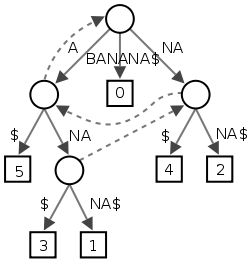
\includegraphics[height=12em]{suffix-tree-banana.png}
\end{center}
\end{columns}
\end{frame}


\begin{frame}[fragile]
  \frametitle{Binary Tree}

  \center{Btree, the default index type}
  \vfill

\begin{columns}[c]
\column{.55\textwidth} 

  \begin{itemize}
  \item Built for speed
  \item \textit{unique} concurrency tricks
  \item Balanced
  \item support function: \texttt{cmp}
  \item operators: \texttt{<= < = > >=}
  \end{itemize}

\column{.45\textwidth}
\begin{center}
  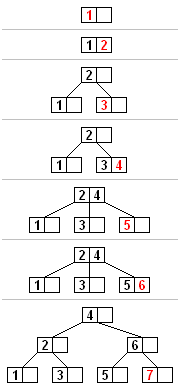
\includegraphics[height=14em]{B_tree_insertion_example.png}
\end{center}
\end{columns}
\end{frame}


\begin{frame}[fragile]
  \frametitle{Generalized Index Search Tree}

  \center{GiST or the Indexing API}
  \vfill

\begin{columns}[c]
\column{.55\textwidth} 

  \begin{itemize}
  \item Built for comfort
  \item Balanced
  \item API: \texttt{consistent}, \texttt{same}, \texttt{union}
  \item API: \texttt{penalty}, \texttt{picksplit}
  \item API: \texttt{compress}, \texttt{decompress}
  \item operators: \texttt{@> <@ \&\& @@ = \&< \&> <<| ...}
  \end{itemize}

\column{.45\textwidth}
\begin{center}
  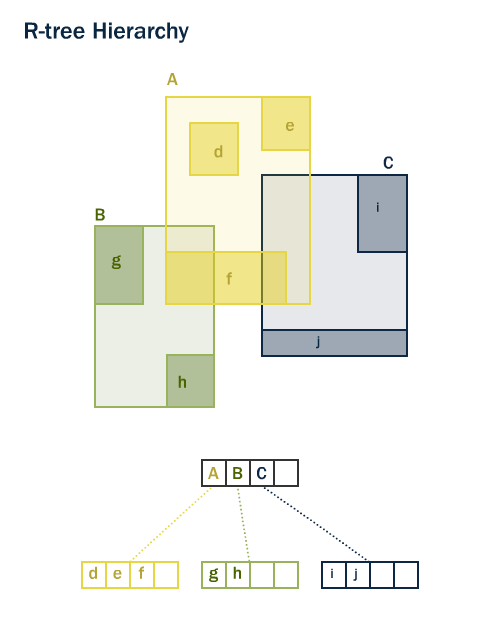
\includegraphics[height=14em]{rtree.png}
\end{center}
\end{columns}
\end{frame}


\begin{frame}[fragile]
  \frametitle{Generalized Inverted iNdex}

  \center{Indexing several pointers per value, inversed cardinality}
  \vfill

\begin{columns}[c]
\column{.55\textwidth} 

  \begin{itemize}
  \item Built for Text Search and Arrays
  \item Balanced
  \item API: \texttt{compare}, \texttt{consistent}
  \item API: \texttt{extractValue}, \texttt{extractQuery}
  \item operators: \texttt{@> <@ \&\& =}
  \end{itemize}

\column{.45\textwidth}
\begin{center}
  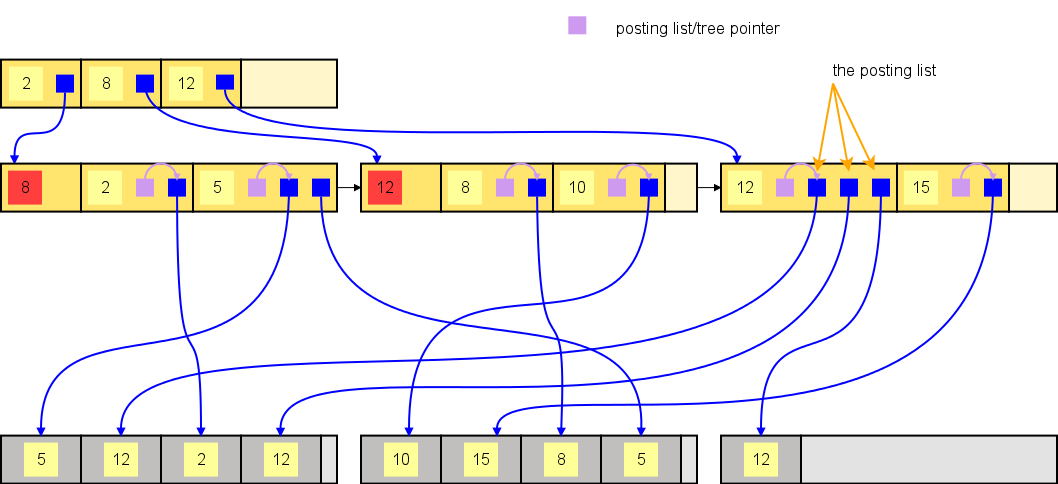
\includegraphics[height=5em]{gin.png}
\end{center}
\end{columns}
\end{frame}

\section{Extensions}

\begin{frame}[fragile]
  \frametitle{Extensions and data types}

\begin{center}
  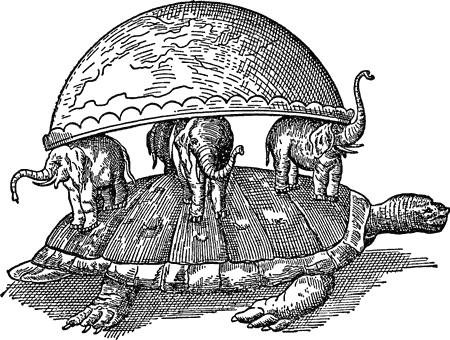
\includegraphics[height=18em]{extensions.png}
\end{center}
\end{frame}

\begin{frame}[fragile]
  \frametitle{Some extensions example}

  \center{46 Contribs, Community extensions, Private ones...}
  \vfill

\begin{columns}[c]

\column{.18\textwidth}
  \begin{itemize}
   \item \alert{hll}
   \item cube
   \item \alert{ltree}
   \item citext
   \item \alert{hstore}
  \end{itemize}

\column{.25\textwidth}
  \begin{itemize}
   \item \alert{earthdistance}
   \item pgq
   \item \alert{pg\_trgm}
   \item wildspeed
   \item \alert{plproxy}
  \end{itemize}

\column{.21\textwidth} 
  \begin{itemize}
   \item PostGIS
   \item \alert{ip4r}
   \item \alert{intarray}
   \item \alert{prefix}
   \item pgfincore
  \end{itemize}

\column{.4\textwidth}
  \begin{itemize}
   \item pgcrypto
   \item pg\_stattuple
   \item pg\_buffercache
   \item pg\_stat\_statements
   \item \alert{pgfincore}
  \end{itemize}

\end{columns}
\end{frame}

\section{IP Ranges with ip4r}

\begin{frame}[fragile]
  \frametitle{IP Ranges, \texttt{ip4r}}

\begin{center}
  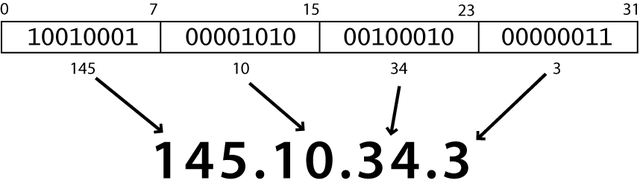
\includegraphics[height=6em]{ip-address.png}
\end{center}
\end{frame}

\begin{frame}[fragile]
  \frametitle{IP Ranges, \texttt{ip4r}}

\begin{columns}
\column{.7\textwidth}
\begin{minted}{postgresql}
table geolite.blocks limit 10;
        iprange        | locid 
-----------------------+-------
 1.0.0.0/24            |    17
 1.0.1.0-1.0.3.255     |    49
 1.0.4.0/23            | 14409
 1.0.6.0/23            |    17
 1.0.8.0/21            |    49
 1.0.16.0/20           | 14614
 1.0.32.0/19           | 47667
 1.0.64.0/18           |   111
 1.0.128.0-1.0.147.255 |   209
 1.0.148.0/24          | 22537
(10 rows)
\end{minted}
\end{columns}
\end{frame}

\begin{frame}[fragile]
  \frametitle{IP Ranges, \texttt{ip4r}, Geolocation}

  \center{PostgreSQL allows using SQL and JOINs to match IP4R with geolocation.}
  \vfill

\begin{columns}
\column{.45\textwidth}
\begin{minted}{postgresql}
 select *
   from geolite.blocks
   join geolite.location
        using(locid)
  where iprange
            >>=
        '74.125.195.147';
\end{minted}
\column{.55\textwidth}
\begin{center}
  
\includegraphics[height=9em]{geolocation-clic.png}
\end{center}
\end{columns}
\end{frame}

\begin{frame}[fragile]
  \frametitle{IP Ranges, \texttt{ip4r}, Geolocation}

  \center{PostgreSQL allows using SQL and JOINs to match IP4R with geolocation.}
  \vfill

\begin{columns}
\column{.45\textwidth}
\begin{minted}{postgresql}
 select *
   from geolite.blocks
   join geolite.location
        using(locid)
  where iprange
            >>=
        '74.125.195.147';
\end{minted}
\column{.55\textwidth}
\begin{minted}{postgresql}
-[ RECORD 1 ]----------------------------
locid      | 2703
iprange    | 74.125.189.24-74.125.255.255
country    | US
region     | CA
city       | Mountain View
postalcode | 94043
location   | (-122.0574,37.4192)
metrocode  | 807
areacode   | 650

Time: 1.335 ms
\end{minted}
\end{columns}
\end{frame}

\section{Earth Distance}

\begin{frame}[fragile]
  \frametitle{Earth Distance}

\begin{center}
  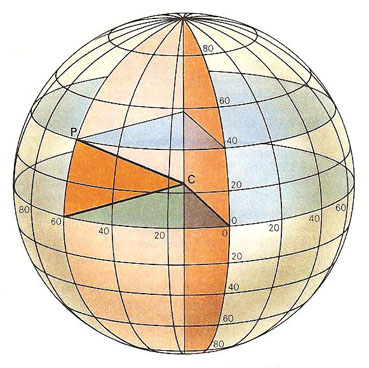
\includegraphics[height=15em]{latitude_and_longitude.jpg}
\end{center}
\end{frame}

\begin{frame}[fragile]
  \frametitle{How Far is The Nearest Pub}

  \center{The \texttt{point} datatype is in-core}
  \vfill

\begin{columns}[c]
\column{.45\textwidth} 

\begin{minted}{postgresql}
#  CREATE TABLE pubnames
   (
     id   bigint,
     pos  POINT,
     name text
   );
\end{minted}  

\column{.55\textwidth}
\begin{center}
  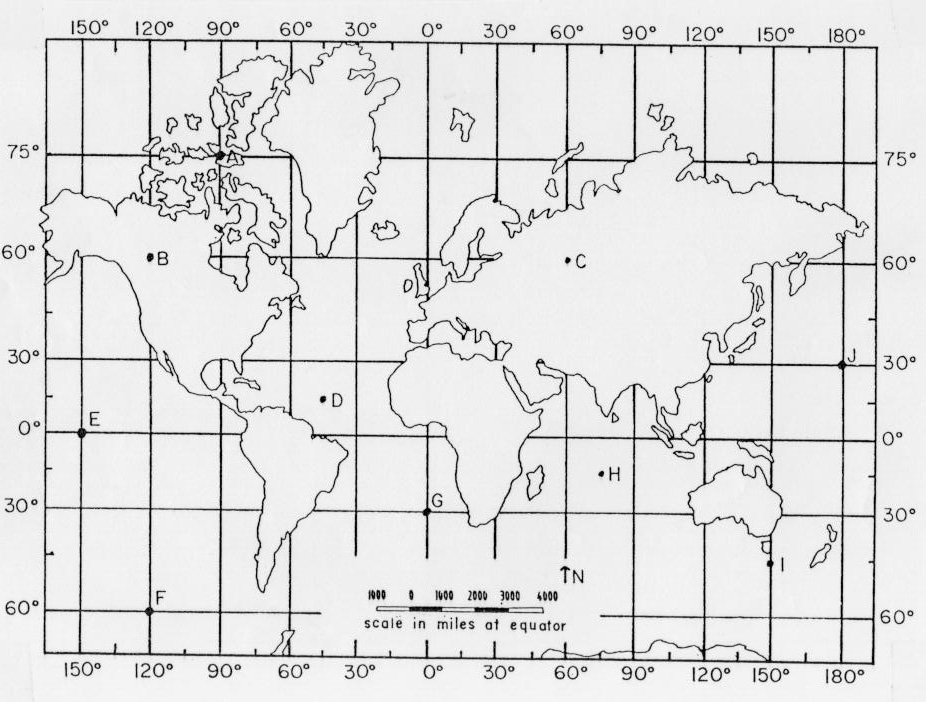
\includegraphics[height=9em]{ltlng.jpg}
\end{center}
\end{columns}
\end{frame}

\begin{frame}[fragile]
  \frametitle{How Far is The Nearest Pub}

\begin{minted}{postgresql}
  select name, pos
    from pubnames
order by pos <-> point(-6.25,53.346)
    limit 3;

          Pub Name          |           pos           
----------------------------+-------------------------
 Ned's                      | (-6.2519967,53.3458267)
 Sub Lounge                 | (-6.2542332,53.3469085)
 O'Neill's of Pearse Street | (-6.2524389,53.3448589)
(3 rows)

Time: 18.679 ms
\end{minted}  
\end{frame}

\begin{frame}[fragile]
  \frametitle{How Far is The Nearest Pub}

\begin{center}
\begin{minted}{postgresql}
CREATE INDEX on pubnames USING GIST(pos);
\end{minted}  
\end{center}
\vfill

\begin{columns}
\column{.65\textwidth}
\begin{minted}{postgresql}
  select name,
         pos
    from pubnames
order by pos <-> point(-0.12,51)
   limit 3;
\end{minted}  

\column{.35\textwidth}
\begin{minted}{postgresql}
  name  |      pos           
--------+--------------
 Ned's  | (-6.25,53.34)
 Sub Lo | (-6.25,53.34)
 O'Neil | (-6.25,53.34)
(3 rows)

Time: 0.849 ms
\end{minted}  
\end{columns}
\end{frame}

\begin{frame}[fragile]
  \frametitle{How Far is The Nearest Pub, in Miles please.}

\begin{minted}{postgresql}
create extension cube;
create extension earthdistance;
\end{minted}  
\vfill

\begin{columns}
\column{.65\textwidth}
\begin{minted}{postgresql}
  select name,
   pos <@> point(-6.25,53.34) miles
    from pubnames
order by pos <-> point(-6.25,53.34)
   limit 3;
\end{minted}  
\column{.35\textwidth}
\begin{minted}{postgresql}
  name  | miles 
--------+-------
 Ned's  |  0.06
 Sub Lo |  0.07
 O'Neil |  0.12
(3 rows)

Time: 1.335 ms
\end{minted}  
\end{columns}
\end{frame}

\begin{frame}[fragile]
  \frametitle{Some pubs far away from here...}

\begin{columns}
\column{.65\textwidth}
\begin{minted}{postgresql}
  select c.name as city,
  pos <@> point(-6.25,53.34) as miles
   from pubnames p,
     lateral (select name
                from cities c
            order by c.pos <-> p.pos
               limit 1) c
 order by pos <-> point(-6.25,53.34)
           desc
    limit 5;
\end{minted}  
\column{.35\textwidth}
\begin{minted}{postgresql}
    city    |  miles       
------------+--------
 Canterbury | 399.44
 Canterbury | 378.91
 Canterbury | 392.08
 Canterbury | 397.30
 Canterbury | 379.68
(5 rows)

Time: 636.445 ms
\end{minted}  
\end{columns}
\end{frame}

\begin{frame}[fragile]
  \frametitle{Geolocation: \texttt{ip4r} meets \text{earthdistance}}

\begin{center}
  
\includegraphics[height=12em]{geolocation.png}
\end{center}
\end{frame}

\begin{frame}[fragile]
  \frametitle{Some pubs nearby... some place...}

\begin{columns}
\column{.5\textwidth}
\begin{minted}{postgresql}
with geoloc as
 (
  select location as l
    from location
    join blocks using(locid)
   where iprange
         >>=
         '212.58.251.195'
 )
  select name,
         pos <@> l miles
    from pubnames, geoloc
order by pos <-> l
   limit 10;
\end{minted}  
\column{.5\textwidth}
\begin{minted}{postgresql}
        name        | miles 
--------------------+-------
 Blue Anchor        | 0.299
 Dukes Head         | 0.360
 Blue Ball          | 0.337
 Bell (aka The Rat) | 0.481
 on the Green       | 0.602
 Fox & Hounds       | 0.549
 Chequers           | 0.712
 Sportsman          | 1.377
 Kingswood Arms     | 1.205
 Tattenham Corner   | 2.007
(10 rows)

Time: 3.275 ms
\end{minted}  
\end{columns}
\end{frame}

\section{Trigrams}

\begin{frame}[fragile]
  \frametitle{Trigrams}

\begin{center}
  
\includegraphics[height=12em]{trigramme.png}
\end{center}
\end{frame}

\begin{frame}[fragile]
  \frametitle{Trigrams and similarity}

  \center{\textit{similar} but not quite \textit{like} the same}
  \vfill

\begin{columns}
\column{.9\textwidth}
\begin{minted}{postgresql}
create extension pg_trgm;

select show_trgm('tomy') as tomy,
       show_trgm('Tomy') as "Tomy",
       show_trgm('tom torn') as "tom torn",
       similarity('tomy', 'tom'),
       similarity('dim', 'tom');

-[ RECORD 1 ]-------------------------------------
tomy       | {"  t"," to","my ",omy,tom}
Tomy       | {"  t"," to","my ",omy,tom}
tom torn   | {"  t"," to","om ",orn,"rn ",tom,tor}
similarity | 0.5
similarity | 0
\end{minted}  
\end{columns}
\end{frame}

\begin{frame}[fragile]
  \frametitle{Trigrams and typos}

  \center{Use your data to help your users out}
  \vfill

\begin{columns}
\column{.5\textwidth}
\begin{minted}{postgresql}
select actor
  from products
 where actor ~* 'tomy';
  actor   
----------


(0 rows)

Time: <unregistered>
\end{minted}  
\column{.5\textwidth}
\begin{minted}{postgresql}
select actor
  from products
 where actor % 'tomy';
  actor   
----------
 TOM TORN
 TOM DAY
(2 rows)

Time: 26.972 ms
\end{minted}  
\end{columns}
\end{frame}

\begin{frame}[fragile]
  \frametitle{Trigrams search indexing}

\begin{minted}{postgresql}
create index on products using gist(actor gist_trgm_ops);
\end{minted}
\vfill

\begin{columns}
\column{.5\textwidth}
\begin{center}
  
\includegraphics[height=9em]{macrex-index.png}
\end{center}
\column{.5\textwidth}
\begin{minted}{postgresql}
select actor
  from products
 where actor % 'tomy';
  actor   
----------
 TOM TORN
 TOM DAY
(2 rows)

Time: 2.695 ms
\end{minted}  
\end{columns}
\end{frame}

\begin{frame}[fragile]
  \frametitle{Trigrams and autocompletion}

  \center{Use your data to help your users out}
  \vfill

\begin{columns}
\column{.9\textwidth}
\begin{minted}{postgresql}
explain (costs off)
 select * from products where actor ~* 'tomy';
                   QUERY PLAN                    
-------------------------------------------------
 Index Scan using products_actor_idx on products
   Index Cond: ((actor)::text ~* 'tomy'::text)
(2 rows)
\end{minted}  
\end{columns}
\end{frame}

\begin{frame}[fragile]
  \frametitle{Trigrams and autocompletion}

  \center{Use your data to help your users out}
  \vfill

\begin{columns}
\column{.5\textwidth}
\begin{minted}{postgresql}
  select actor
    from products
   where actor % 'fran'
order by actor <-> 'fran'
   limit 10;
\end{minted}  
\column{.5\textwidth}
\begin{minted}{postgresql}
    actor     
--------------
 FRANK HAWKE
 FRANK BERRY
 FRANK POSEY
 FRANK HAWKE
 FRANCES DEE
 FRANK LEIGH
 FRANCES DAY
 FRANK FOSTER
 FRANK HORNE
 FRANK TOMEI
(10 rows)

Time: 2.960 ms
\end{minted}  
\end{columns}
\end{frame}

\section{Indexing Tag Searches}

\begin{frame}[fragile]
  \frametitle{Advanced Array Indexing with \texttt{intarray}}

\begin{center}
  
\includegraphics[height=15em]{wordpres-seo-categories-tags.jpg}
\end{center}
\end{frame}

\begin{frame}[fragile]
  \frametitle{Last.fm allows users to tag tracks}

\begin{columns}
\column{.4\textwidth}
\begin{minted}{postgresql}
  select t.tag,
         count(tt.tid) n
    from tid_tag tt
    join tags t
      on tt.tag = t.rowid
   where t.tag ~* 'setzer'
group by t.tag;
\end{minted}  
\column{.6\textwidth}
\begin{minted}{postgresql}
             tag             |  n 
-----------------------------+----
 the brian setzer orchestra  |  1
 setzer                      | 13
 rockabilly setzer style     |  4
 setzer is a true guitarhero |  9
 brian setzer orchestra      |  3
 brian setzer is god         |  1
 brian setzer                |  1
 brain setzer orchestra      |  2
(8 rows)

time: 644.826 ms
\end{minted}  
\end{columns}
\end{frame}

\begin{frame}[fragile]
  \frametitle{Last.fm allows users to tag tracks}

\begin{minted}{postgresql}
create extension intarray;
\end{minted}
\vfill

\begin{columns}
\column{.7\textwidth}
\begin{minted}{postgresql}
  select tt.tid,
         array_agg(tags.rowid) tags
    from tags
         join tid_tag tt
           on tags.rowid = tt.tag
group by tt.tid
   limit 3;
\end{minted}  
\column{.3\textwidth}
\begin{minted}{postgresql}
 tid |   tags    
-----+-----------
   1 | {1,2}
   2 | {3,4}
   3 | {5,6,7,8}
(3 rows)

time: 942.074 ms
\end{minted}  
\end{columns}
\end{frame}

\begin{frame}[fragile]
  \frametitle{Prepare for \texttt{intarray} indexing}

  \center{Denormalize the data set thanks to PostgreSQL Arrays}
  \vfill
  
\begin{minted}{postgresql}
create table track_tags as
   select tt.tid, array_agg(tags.rowid) as tags
     from tags join tid_tag tt on tags.rowid = tt.tag
 group by tt.tid;

create index on track_tags using gin(tags gin__int_ops);
\end{minted}  
\end{frame}

\begin{frame}[fragile]
  \frametitle{Search for several tags at once}

  \center{Intersection of multiple criteria}
  \vfill

\begin{columns}
\column{.6\textwidth}
\begin{minted}{postgresql}
select array_agg(rowid)
  from tags
 where tag = 'blues'
    or tag = 'rhythm and blues';
\end{minted}  
\column{.4\textwidth}
\begin{minted}{postgresql}
 array_agg 
-----------
 {3,739}
(1 row)

time: 0.684 ms
\end{minted}  
\end{columns}
\end{frame}

\begin{frame}[fragile]
  \frametitle{The \texttt{query\_int} data type}

  \center{\texttt{intarray} has powerful indexing and searching facilities}
  \vfill

\begin{columns}
\column{.6\textwidth}
\begin{minted}{postgresql}
select format('(%s)',
        array_to_string(
         array_agg(rowid), '&')
       )::query_int as query
  from tags
 where tag = 'blues'
    or tag = 'rhythm and blues';
\end{minted}  
\column{.4\textwidth}
\begin{minted}{postgresql}
  query  
---------
 3 & 739
(1 row)

time: 0.747 ms
\end{minted}  
\end{columns}
\end{frame}

\begin{frame}[fragile]
  \frametitle{Putting it all together}

\begin{columns}
\column{.6\textwidth}
\begin{minted}{postgresql}
with t(query) as (
 select format('(%s)',
         array_to_string(
          array_agg(rowid), '&')
        )::query_int as query
   from tags
  where tag = 'blues'
     or tag = 'rhythm and blues'
)
 select track.tid
   from track_tags tt
   join tids track
     on tt.tid = track.rowid, t
  where tt.tags @@ t.query
  limit 10;
\end{minted}  
\column{.4\textwidth}
\begin{minted}{postgresql}
        tid         
--------------------
 TRCJLCC12903CBF4AE
 TRCIFOV128F92F6F4C
 TRCYUVJ128F425C8F1
 TRCNTFO128F92F6564
 TRCDRGT12903CE64BF
 TRCWAED128F42A837B
 TRCWFEM128F9320F94
 TRCQCQH128F932E707
 TRCUMTA12903CD67EE
 TRJJYUT12903CFB13B
(10 rows)

Time: 7.630 ms
\end{minted}  
\end{columns}
\end{frame}

\section{HStore}

\begin{frame}[fragile]
  \frametitle{HStore}

\begin{center}
  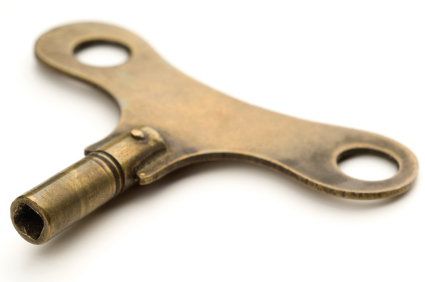
\includegraphics[height=15em]{clock-key.jpg}
\end{center}
\end{frame}

\begin{frame}[fragile]
  \frametitle{HStore: NoSQL meets PostgreSQL}

\begin{columns}
\column{.7\textwidth}
  \begin{itemize}
   \item Key-Value Store
   \item Denormlisation
   \item Indexing (GiST, GIN)
   \item Operators
   \item SQL
  \end{itemize}  
\column{.3\textwidth}
\begin{center}
  
\includegraphics[height=6em]{hstore.png}
\end{center}
\end{columns}
\end{frame}

\begin{frame}[fragile]
  \frametitle{HStore: NoSQL meets PostgreSQL}

\begin{columns}
\column{.7\textwidth}
\begin{minted}{postgresql}
create table preferences
(
  email       text      primary key,
  language    text,
  timezone    text,
  properies  hstore
);
\end{minted}  
\column{.3\textwidth}
\begin{center}
  
\includegraphics[height=6em]{hstore.png}
\end{center}
\end{columns}
\end{frame}

\begin{frame}[fragile]
  \frametitle{HStore: NoSQL meets PostgreSQL}

\begin{minted}{postgresql}
INSERT INTO preferences
VALUES
  ('dimitri@2ndQuadrant.fr', 'fr_FR', 'Europe/Paris',
   'skills => PostgreSQL,
    Extensions => "prefix, base64, pgextwlist, preprepare",
    Software => "pgloader"'),

  ('simon@2ndQuadrant.com', 'en_UK', 'Europe/London',
   'skills => "PostgreSQL, Replication",
    Software => "PostgreSQL, repmgr, pg_standby"');

INSERT 0 2
\end{minted}  
\end{frame}

\begin{frame}[fragile]
  \frametitle{HStore: NoSQL meets PostgreSQL}

\begin{minted}{postgresql}
~# select * from preferences;
-[ RECORD 1 ]------------------------------------------------------
email     | dimitri@2ndQuadrant.fr
language  | fr_FR
timezone  | Europe/Paris
properies | "skills"=>"PostgreSQL",
            "Software"=>"pgloader",
            "Extensions"=>"prefix, base64, pgextwlist, preprepare"
-[ RECORD 2 ]-------------------------------------------
email     | simon@2ndQuadrant.com
language  | en_UK
timezone  | Europe/London
properies | "skills"=>"PostgreSQL, Replication",
            "Software"=>"PostgreSQL, repmgr, pg_standby"
\end{minted}  
\end{frame}

\begin{frame}[fragile]
  \frametitle{HStore: NoSQL meets PostgreSQL}

\begin{columns}
\column{.8\textwidth}
\begin{minted}{postgresql}
~# select email
     from preferences
    where properies ? 'Extensions';
         email          
------------------------
 dimitri@2ndQuadrant.fr
(1 row)
\end{minted}  
\end{columns}
\end{frame}

\begin{frame}[fragile]
  \frametitle{HStore: NoSQL meets PostgreSQL}

\begin{columns}
\column{.8\textwidth}
\begin{minted}{postgresql}
~# select email
     from preferences
    where (properies -> 'skills') ~ 'PostgreSQL';
         email          
------------------------
 dimitri@2ndQuadrant.fr
 simon@2ndQuadrant.com
(2 rows)
\end{minted}  
\end{columns}
\end{frame}

\begin{frame}[fragile]
  \frametitle{HStore and Parametrized Triggers}

\begin{center}
  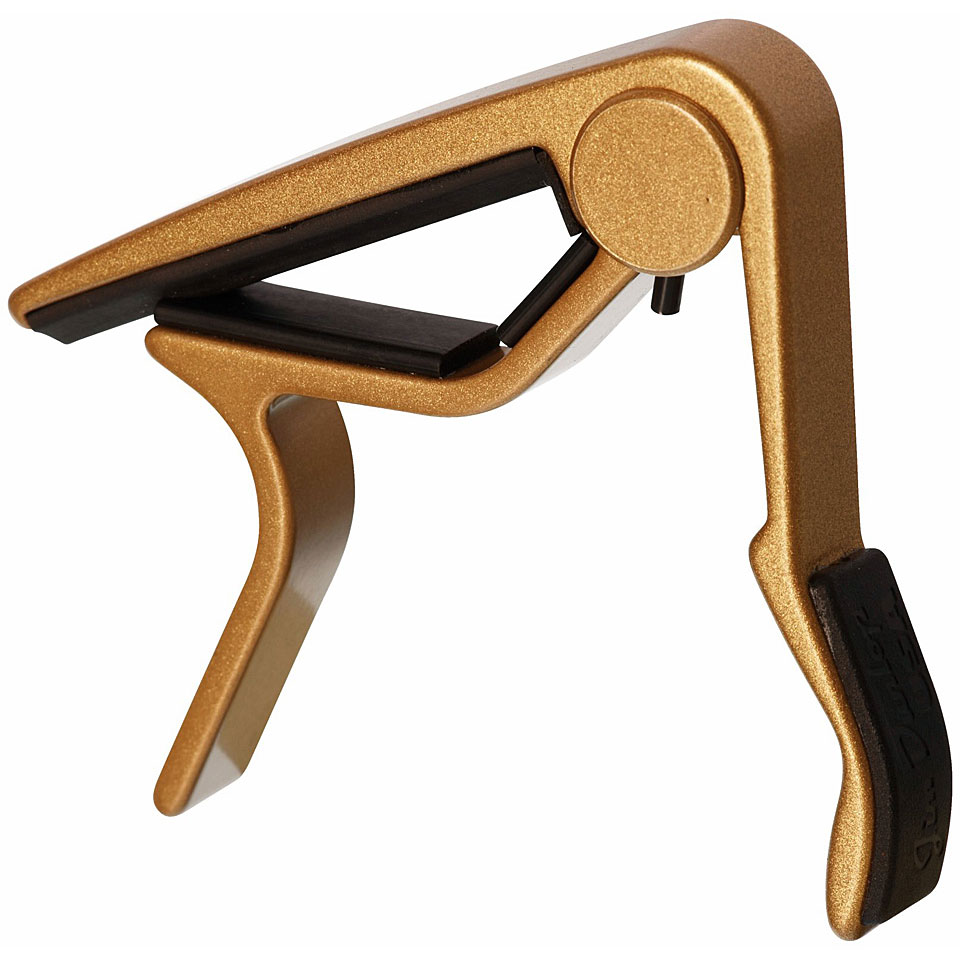
\includegraphics[height=15em]{dunlop-trigger-84fg-gold.jpg}
\end{center}
\end{frame}

\begin{frame}[fragile]
  \frametitle{Compute \textit{duration} in a before trigger}

  \center{We need a table and some data}
  \vfill
  
\begin{columns}
\column{.8\textwidth}
\begin{minted}{postgresql}
create table foo
(
  id       serial      primary key,
  d_start  timestamptz default now(),
  d_end    timestamptz,
  duration interval
);

insert into foo(d_start, d_end)
     select now() - 10 * random() * interval '1 min',
            now() + 10 * random() * interval '1 min'
       from generate_series(1, 10);
\end{minted}  
\end{columns}
\end{frame}

\begin{frame}[fragile]
  \frametitle{Populating an \texttt{hstore} from a \texttt{record}}

  \center{Filling in a column when the name is a parameter}
  \vfill
  
\begin{columns}
\column{.8\textwidth}
\begin{minted}{postgresql}
select (foo #= hstore('duration', '10 mins')).*
  from foo
  limit 1;

-[ RECORD 1 ]---------------------------
id       | 1
d_start  | 2013-10-24 18:57:36.725212+02
d_end    | 2013-10-24 19:04:56.171473+02
duration | 00:10:00
\end{minted}  
\end{columns}
\end{frame}

\begin{frame}[fragile]
  \frametitle{The \texttt{hstore} based \textit{parametrized} trigger}

\begin{columns}
\column{.8\textwidth}
\begin{minted}{postgresql}
create or replace function tg_duration()
 returns trigger
 language plpgsql
as '
declare
   hash hstore := hstore(NEW);
   duration interval;
begin
   duration :=  (hash -> TG_ARGV[1])::timestamptz
              - (hash -> TG_ARGV[0])::timestamptz;

   NEW := NEW #= hstore(TG_ARGV[2], duration::text);

   RETURN NEW;
end;
';
\end{minted}
\end{columns}
\end{frame}

\begin{frame}[fragile]
  \frametitle{Installing the trigger}

  \center{To be able to modify what's inserted we need a \texttt{before} trigger}
  \vfill

\begin{columns}
\column{.8\textwidth}
\begin{minted}{postgresql}
    create trigger compute_duration
     before insert on foo
          for each row
 execute procedure tg_duration('d_start',
                               'd_end',
                               'duration');
\end{minted}  
\end{columns}
\end{frame}

\begin{frame}[fragile]
  \frametitle{Using the trigger: watch the \texttt{duration}}

\begin{columns}
\column{.6\textwidth}
\begin{minted}[linenos]{postgresql}
truncate foo;
insert into foo(d_start, d_end)
     select now()
          - 10 * random()
               * interval '1 min',
            now()
          + 10 * random()
            * interval '1 min'
       from generate_series(1, 10);
\end{minted}  
\column{.4\textwidth}
\begin{minted}{postgresql}
select duration
  from foo;
    duration     
-----------------
 00:03:48.003135
 00:10:57.727407
 00:01:13.637183
 00:10:33.820578
 00:13:11.607287
 00:04:41.224213
 00:08:26.842229
 00:12:16.630843
 00:09:51.418547
 00:08:52.968195
(10 rows)
\end{minted}  
\end{columns}
\end{frame}

\section{plproxy}

\begin{frame}[fragile]
  \frametitle{\texttt{PL/Proxy}}

\begin{center}
  
\includegraphics[height=18em]{distribution.jpg}
\end{center}
\end{frame}

\begin{frame}[fragile]
  \frametitle{\texttt{PL/Proxy}}

  \center{PL/Proxy is all about \textit{Sharding}}
  \vfill
  \vfill
  \begin{center}
    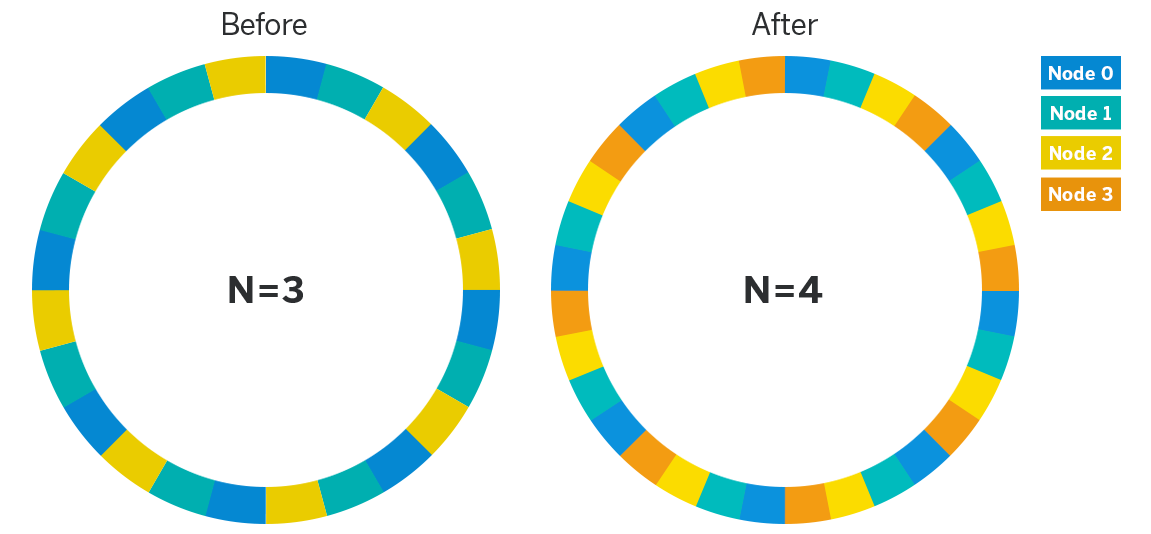
\includegraphics[height=9em]{riak_nodes.png}
  \end{center}
  \center{We're going to use it for \textit{Remote Procedure Call}}
  \vfill
\end{frame}

\begin{frame}[fragile]
  \frametitle{Classic Auditing}

\begin{columns}
\column{.4\textwidth}
\begin{minted}{postgresql}
create table example
 (
   id serial,
   f1 text,
   f2 text
 );
\end{minted}  
\column{.6\textwidth}
\begin{minted}{postgresql}
create table audit
 (
  change_date timestamptz
              default now(),
  before hstore,
  after  hstore
 );
\end{minted}  
\end{columns}
\end{frame}

\begin{frame}[fragile]
  \frametitle{Classic trigger based Auditing}

\begin{columns}
\column{.8\textwidth}
\begin{minted}{postgresql}
~# begin;
~*# update example set f1 = 'b' where id = 1;
~*# rollback;

~# select * from audit;
 change_date | before | after 
-------------+--------+-------
(0 rows)
\end{minted}  
\end{columns}
\end{frame}

\begin{frame}[fragile]
  \frametitle{Seting up \texttt{PL/Proxy}}

\begin{columns}
\column{.8\textwidth}
\begin{minted}{postgresql}
create extension plproxy;

       create server local
foreign data wrapper plproxy
             options (p0 'dbname=dim');

create user mapping
                for public
             server local
            options (user 'dim');
\end{minted}  
\end{columns}
\end{frame}

\begin{frame}[fragile]
  \frametitle{\texttt{PL/Proxy}: Basic Testing}

\begin{columns}
\column{.5\textwidth}
\begin{minted}{postgresql}
create function test_proxy
           (i int)
   returns int
  language plproxy
as '
  cluster ''local'';
  select i;
';
\end{minted}  

\column{.5\textwidth}
\begin{minted}{postgresql}
select test_proxy(1);
 test_proxy 
------------
          1
(1 row)

Time: 0.866 ms
\end{minted}  
\end{columns}
\end{frame}

\begin{frame}[fragile]
  \frametitle{Implementing Autonomous Transactions for Auditing}

\begin{center}
  
\includegraphics[height=9em]{Stealth-Remote-Trigger.jpg}
\end{center}
\end{frame}

\begin{frame}[fragile]
  \frametitle{Trigger Functions 1/3: the trigger}

\begin{columns}
\column{.8\textwidth}
\begin{minted}{postgresql}
create function audit_trigger()
  returns trigger
  language plpgsql
as '
begin
  perform audit_proxy(old, new);
  return new;
end;
';
\end{minted}
\end{columns}
\end{frame}

\begin{frame}[fragile]
  \frametitle{Trigger Functions 2/3: the proxy}

\begin{columns}
\column{.8\textwidth}
\begin{minted}{postgresql}
create function audit_proxy
 (
  old example,
  new example
 )
  returns void
  language plproxy
as '
  cluster ''local'';
  target audit;
';
\end{minted}
\end{columns}
\end{frame}

\begin{frame}[fragile]
  \frametitle{Trigger Functions 3/3: the implementation}

\begin{columns}
\column{.8\textwidth}
\begin{minted}{postgresql}
create function audit
 (
  old example,
  new example
 )
  returns void
  language SQL
as '
  INSERT INTO audit(before, after)
       SELECT hstore(old), hstore(new);   
';
\end{minted}  
\end{columns}
\end{frame}

\begin{frame}[fragile]
  \frametitle{Trigger Definition}

\begin{columns}
\column{.8\textwidth}
\begin{minted}{postgresql}
      drop trigger if exists audit on example;

    create trigger audit
      after update on example
          for each row
          -- careful, defaults to FOR EACH STATEMENT!
 execute procedure audit_trigger();
\end{minted}  
\end{columns}
\end{frame}

\begin{frame}[fragile]
  \frametitle{Autonomous Auditing Transaction}

\begin{columns}
\column{.8\textwidth}
\begin{minted}{postgresql}
~# begin;
BEGIN

~*# update example set f1 = 'b' where id = 1;
UPDATE 1

~*# rollback;
ROLLBACK
\end{minted}  
\end{columns}
\end{frame}

\begin{frame}[fragile]
  \frametitle{Autonomous Auditing Tranasction}

  \center{We did \texttt{ROLLBACK;} the transaction}
  \vfill

\begin{columns}
\column{.8\textwidth}
\begin{minted}{postgresql}
~# select change_date,
          before,
          after,
          after - before as diff
     from audit;
-[ RECORD 1 ]--------------------------------
change_date | 2013-10-14 14:29:09.685105+02
before      | "f1"=>"a", "f2"=>"a", "id"=>"1"
after       | "f1"=>"b", "f2"=>"a", "id"=>"1"
diff        | "f1"=>"b"
\end{minted}  
\end{columns}
\end{frame}

\section{HyperLogLog}

\begin{frame}[fragile]
  \frametitle{HyperLogLog}

  \center{State of The Art Cardinality Estimation Algorithm}
  \vfill

\begin{center}
  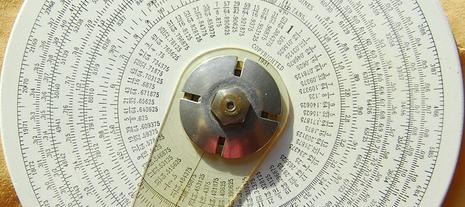
\includegraphics[height=12em]{cardinality1.jpg}
\end{center}
\end{frame}

\begin{frame}[fragile]
  \frametitle{Creating the unique visitors tracking table}

\begin{minted}{postgresql}
CREATE EXTENSION hll;

-- Create the destination table
CREATE TABLE daily_uniques (
    DATE            DATE UNIQUE,
    users           hll
);

-- Our first aggregate update
UPDATE daily_uniques
   SET users = hll_add(users,
                 hll_hash_text('123.123.123.123'))
 WHERE date = current_date;
\end{minted}  
\end{frame}

\begin{frame}[fragile]
  \frametitle{Production ready updates}

\begin{minted}{postgresql}
--
-- First upload a new batch, e.g. using
--    CREATE TEMP TABLE new_batch as VALUES(), (), ...;
--
WITH hll(agg) AS (
 SELECT hll_add_agg(hll_hash_text(value))
   FROM new_batch
)
 UPDATE daily_uniques
    SET users = CASE WHEN hll.agg IS NULL THEN users
                     ELSE hll_union(users, hll.agg)
                 END
   FROM hll
  WHERE date = current_date;
\end{minted}  
\end{frame}

\begin{frame}[fragile]
  \frametitle{Daily Reporting}

\begin{columns}
\column{.5\textwidth}
\begin{minted}{postgresql}
with stats as (
  select date,
         #users as daily,

         #hll_union_agg(users)
         over() as total

    from daily_uniques
)
  select date,
         daily,
         daily/total*100
    from stats
order by date;
\end{minted}  
\column{.5\textwidth}
\begin{minted}{postgresql}
    date    | daily  | percent 
------------+--------+---------
 2013-02-22 | 401677 |   25.19
 2013-02-23 | 660187 |   41.41
 2013-02-24 | 869980 |   54.56
 2013-02-25 | 154996 |    9.72
(4 rows)
\end{minted}  
\end{columns}
\end{frame}

\begin{frame}[fragile]
  \frametitle{Monthly Reporting}

\begin{columns}
\column{.65\textwidth}
\begin{minted}{postgresql}
  select to_char(date, 'YYYY/MM'),
         #hll_union_agg(users)
    from daily_uniques
group by 1;
\end{minted}  
\column{.35\textwidth}
\begin{minted}{postgresql}     
  month  | monthly 
---------+---------
 2013/02 | 1960380
(1 row)
\end{minted}  
\end{columns}
\end{frame}

\section{Background Workers}

\begin{frame}[fragile]
  \frametitle{New in 9.3: Background Workers}

\begin{center}
  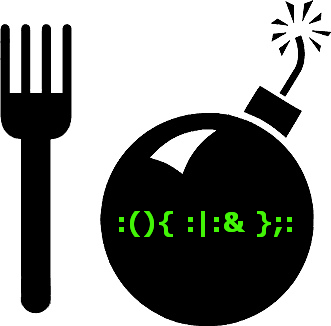
\includegraphics[height=9em]{fork-bomb.png}
\end{center}
\end{frame}

\begin{frame}[fragile]
  \frametitle{New in 9.3: Background Workers}

  \center{Start autonomous user processes within the database server}
  \vfill

\begin{columns}
\column{.7\textwidth}
  \begin{itemize}
  \item Job Scheduler (autovacuum like maintainance)
  \item PGQ Ticker
  \item Replication Tasks
  \item Parallel Queries
  \end{itemize}
\column{.3\textwidth}
\begin{center}
  
\includegraphics[height=6em]{clock.png}
\end{center}
\end{columns}
\end{frame}

\begin{frame}[fragile]
  \frametitle{Background Workers C API}

\begin{minted}{c}
void _PG_init(void)
{
  BackgroundWorker worker;

  worker.bgw_flags = BGWORKER_SHMEM_ACCESS |
       BGWORKER_BACKEND_DATABASE_CONNECTION;
  worker.bgw_start_time   = BgWorkerStart_RecoveryFinished;
  worker.bgw_main         = worker_spi_main;
  worker.bgw_sighup       = worker_spi_sighup;
  worker.bgw_sigterm      = worker_spi_sigterm;
  worker.bgw_name         = "count relations";
  worker.bgw_restart_time = BGW_NEVER_RESTART;
  worker.bgw_main_arg     = NULL;
  RegisterBackgroundWorker(&worker);

  BackgroundWorkerInitializeConnection("dbname", "username");
}
\end{minted}
\end{frame}

\begin{frame}[fragile]
  \frametitle{Background Workers C API}

  \center{\texttt{bgw\_start\_time}}
  \vfill

  \begin{itemize}
  \item \texttt{BgWorkerStart\_PostmasterStart}
  \item \texttt{BgWorkerStart\_ConsistentState}
  \item \texttt{BgWorkerStart\_RecoveryFinished}
  \end{itemize}
\end{frame}

\begin{frame}[fragile]
  \frametitle{Background Workers and SPI}

\begin{minted}{c}
StartTransactionCommand();
SPI_connect();
PushActiveSnapshot(GetTransactionSnapshot());

/* build query, might be static string */

SPI_execute(query, true/false /* read only */, 0);

/* process query results */

SPI_finish();
PopActiveSnapshot();
CommitTransactionCommand();
\end{minted}
\end{frame}

\begin{frame}[fragile]
  \frametitle{New in 9.3: Background Workers}

  \center{Can request \textit{shared memory}, server must be restarted.}
  \vfill

\begin{minted}{ini}
shared_preload_libraries = 'count_relations'
\end{minted}
\end{frame}

\section{base36}

\begin{frame}[fragile]
  \frametitle{Extensions: Let's make a new one!}

\begin{center}
  
\includegraphics[height=18em]{extension-update.png}
\end{center}
\end{frame}

\begin{frame}[fragile]
  \frametitle{A new integer data type: \texttt{base36}}

  \center{Internally store \texttt{bigint}, reuse \textit{internals}}
  \vfill

  \begin{center}
    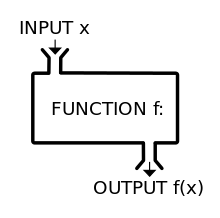
\includegraphics[height=6em]{input-output.png}
  \end{center}

  \begin{center}
    Only code the \textit{input/output} functions, in \texttt{C}
  \end{center}

\end{frame}

\begin{frame}[fragile]
  \frametitle{A new integer data type: \texttt{base36}}

  \begin{minted}{postgresql}
    create extension base36;
  \end{minted}  
  \vfill

\begin{columns}
\column{.25\textwidth}
\begin{minted}{postgresql}
  i | x    
 ---+----
  0 | 0
  1 | 1
  2 | 2
  3 | 3
  4 | 4
  5 | 5
  6 | 6
  7 | 7
  8 | 8
  9 | 9
 10 | A
\end{minted}  
\column{.25\textwidth}
\begin{minted}{postgresql}     
    i   |   x    
 -------+------
  10000 | 7PS
  10001 | 7PT
  10002 | 7PU
  10003 | 7PV
  10004 | 7PW
  10005 | 7PX
  10006 | 7PY
  10007 | 7PZ
  10008 | 7Q0
  10009 | 7Q1
  10010 | 7Q2
\end{minted}  
\column{.50\textwidth}
\begin{minted}{postgresql}     
      i     |   x    
 -----------+--------
  100000000 | 1NJCHS
  100000001 | 1NJCHT
  100000002 | 1NJCHU
  100000003 | 1NJCHV
  100000004 | 1NJCHW
  100000005 | 1NJCHX
  100000006 | 1NJCHY
  100000007 | 1NJCHZ
  100000008 | 1NJCI0
  100000009 | 1NJCI1
  100000010 | 1NJCI2
\end{minted}  
\end{columns}
\end{frame}

\begin{frame}[fragile]
  \frametitle{Input Output Functions}

\begin{minted}{postgresql}
CREATE OR REPLACE FUNCTION base36_in(cstring)
RETURNS base36
AS '$libdir/base36'
LANGUAGE C IMMUTABLE STRICT;

CREATE OR REPLACE FUNCTION base36_out(base36)
RETURNS cstring
AS '$libdir/base36'
LANGUAGE C IMMUTABLE STRICT;
\end{minted}
\end{frame}

\begin{frame}[fragile]
  \frametitle{Input Output Functions}

\begin{minted}{postgresql}
CREATE OR REPLACE FUNCTION base36_recv(internal)
RETURNS base36
AS '$libdir/base36'
LANGUAGE C IMMUTABLE STRICT;

CREATE OR REPLACE FUNCTION base36_send(base36)
RETURNS bytea
AS '$libdir/base36'
LANGUAGE C IMMUTABLE STRICT;
\end{minted}
\end{frame}

\begin{frame}[fragile]
  \frametitle{Some C code}

\begin{minted}{c}
#include "postgres.h"

#ifndef PG_VERSION_NUM
#error "Unsupported too old PostgreSQL version"
#endif

#if  PG_VERSION_NUM / 100 != 903 \
  && PG_VERSION_NUM / 100 != 904
#error "Unknown or unsupported PostgreSQL version"
#endif

PG_MODULE_MAGIC;
\end{minted}
\end{frame}

\begin{frame}[fragile]
  \frametitle{Some C code}

\begin{minted}{c}
static inline
base36 base36_from_str(const char *str)
{
  /* ... C code here ... */
}

static inline
char *base36_to_str(base36 c)
{
  /* ... C code here ... */
}
\end{minted}
\end{frame}

\begin{frame}[fragile]
  \frametitle{Interfacing with PostgreSQL}

\begin{minted}{c}
Datum base36_in(PG_FUNCTION_ARGS);
Datum base36_out(PG_FUNCTION_ARGS);
Datum base36_recv(PG_FUNCTION_ARGS);
Datum base36_send(PG_FUNCTION_ARGS);
Datum base36_cast_to_text(PG_FUNCTION_ARGS);
Datum base36_cast_from_text(PG_FUNCTION_ARGS);
Datum base36_cast_to_bigint(PG_FUNCTION_ARGS);
Datum base36_cast_from_bigint(PG_FUNCTION_ARGS);
\end{minted}
\end{frame}

\begin{frame}[fragile]
  \frametitle{Interfacing with PostgreSQL}

\begin{minted}{c}
PG_FUNCTION_INFO_V1(base36_in);
Datum
base36_in(PG_FUNCTION_ARGS)
{
    char *str = PG_GETARG_CSTRING(0);
    PG_RETURN_INT64(base36_from_str(str));
}

PG_FUNCTION_INFO_V1(base36_out);
Datum
base36_out(PG_FUNCTION_ARGS)
{
  base36 c = PG_GETARG_INT64(0);
  PG_RETURN_CSTRING(base36_to_str(c));
}
\end{minted}
\end{frame}

\begin{frame}[fragile]
  \frametitle{\texttt{CREATE TYPE}}

\begin{minted}[]{postgresql}
CREATE TYPE base36 (
        INPUT          = base36_in,
        OUTPUT         = base36_out,
        RECEIVE        = base36_recv,
        SEND           = base36_send,
        LIKE           = bigint,
        CATEGORY       = 'N'
);
COMMENT ON TYPE base36
     IS 'bigint written in base36: [0-9A-Z]+';
\end{minted}
\end{frame}

\begin{frame}[fragile]
  \frametitle{A minimum amount of \texttt{CAST}}

\begin{columns}
\column{.50\textwidth}
\begin{minted}{postgresql}
CREATE FUNCTION text(base36)
RETURNS text
AS '$libdir/base36',
   'base36_cast_to_text'
LANGUAGE C IMMUTABLE STRICT;

CREATE CAST (text as base36)
  WITH FUNCTION base36(text)
    AS IMPLICIT;
\end{minted}  
\column{.50\textwidth}
\begin{minted}{postgresql}
CREATE CAST (base36 as text)
  WITH FUNCTION text(base36);

CREATE CAST (bigint as base36)
    WITHOUT FUNCTION
         AS IMPLICIT;
CREATE CAST (base36 as bigint)
    WITHOUT FUNCTION
         AS IMPLICIT;
\end{minted}
\end{columns}
\end{frame}

\begin{frame}[fragile]
  \frametitle{Reuse \textit{internals}: comparison functions}

\begin{minted}{postgresql}
CREATE OR REPLACE FUNCTION base36_eq(base36, base36) 
RETURNS boolean LANGUAGE internal IMMUTABLE AS 'int8eq';

CREATE OR REPLACE FUNCTION base36_ne(base36, base36) 
RETURNS boolean LANGUAGE internal IMMUTABLE AS 'int8ne';

CREATE OR REPLACE FUNCTION base36_lt(base36, base36) 
RETURNS boolean LANGUAGE internal IMMUTABLE AS 'int8lt';

CREATE OR REPLACE FUNCTION base36_le(base36, base36) 
RETURNS boolean LANGUAGE internal IMMUTABLE AS 'int8le';
\end{minted}
\end{frame}

\begin{frame}[fragile]
  \frametitle{Reuse \textit{internals}: comparison functions}

\begin{minted}{postgresql}
CREATE OR REPLACE FUNCTION base36_gt(base36, base36) 
RETURNS boolean LANGUAGE internal IMMUTABLE AS 'int8gt';

CREATE OR REPLACE FUNCTION base36_ge(base36, base36) 
RETURNS boolean LANGUAGE internal IMMUTABLE AS 'int8ge';

CREATE OR REPLACE FUNCTION base36_cmp(base36, base36) 
RETURNS integer LANGUAGE internal IMMUTABLE AS 'btint8cmp';
\end{minted}
\end{frame}

\begin{frame}[fragile]
  \frametitle{Register operators}

\begin{minted}{postgresql}
CREATE OPERATOR = (
          LEFTARG = base36,
         RIGHTARG = base36,
        PROCEDURE = base36_eq,
       COMMUTATOR = '=',
          NEGATOR = '<>',
         RESTRICT = eqsel,
             JOIN = eqjoinsel
);
COMMENT ON OPERATOR =(base36, base36) IS 'equals?';
\end{minted}
\end{frame}

\begin{frame}[fragile]
  \frametitle{Add in \texttt{btree} index support, stolen from \texttt{bigint}}

\begin{minted}{postgresql}
CREATE OPERATOR CLASS btree_base36_ops
DEFAULT FOR TYPE base36 USING btree
AS
        OPERATOR        1       <  ,
        OPERATOR        2       <= ,
        OPERATOR        3       =  ,
        OPERATOR        4       >= ,
        OPERATOR        5       >  ,
        FUNCTION        1       base36_cmp(base36, base36);
\end{minted}
\end{frame}

\begin{frame}[fragile]
  \frametitle{Packaging an extension}

\begin{center}
  
\includegraphics[height=12em]{software-upgrade.png}
\end{center}
\end{frame}

\begin{frame}[fragile]
  \frametitle{Packaging an extension}

  \center{We need a Makefile}
  \vfill

\begin{minted}{make}
EXTENSION   = base36
MODULES     = base36
DATA        = base36--1.0.sql base36.control

LDFLAGS=-lrt

PG_CONFIG ?= pg_config
PGXS = $(shell $(PG_CONFIG) --pgxs)
include $(PGXS)
\end{minted}
\end{frame}

\begin{frame}[fragile]
  \frametitle{Installing an extension}

\begin{minted}{console}
$ make install
/usr/local/bin/ccache /usr/bin/gcc -O2 -Wall -Wmissing-prototypes -Wpointer-arith -Wdeclaration-after-statement -Wendif-labels -Wmissing-format-attribute -Wformat-security -fno-strict-aliasing -fwrapv -g  -I. -I./ -I/Users/dim/pgsql/ddl/include/server -I/Users/dim/pgsql/ddl/include/internal   -c -o base36.o base36.c -MMD -MP -MF .deps/base36.Po
/usr/local/bin/ccache /usr/bin/gcc -O2 -Wall -Wmissing-prototypes -Wpointer-arith -Wdeclaration-after-statement -Wendif-labels -Wmissing-format-attribute -Wformat-security -fno-strict-aliasing -fwrapv -g  -L/Users/dim/pgsql/ddl/lib -Wl,-dead_strip_dylibs   -bundle -bundle_loader /Users/dim/pgsql/ddl/bin/postgres -o base36.so base36.o
/bin/sh /Users/dim/pgsql/ddl/lib/pgxs/src/makefiles/../../config/install-sh -c -d '/Users/dim/pgsql/ddl/share/extension'
/bin/sh /Users/dim/pgsql/ddl/lib/pgxs/src/makefiles/../../config/install-sh -c -d '/Users/dim/pgsql/ddl/share/extension'
/bin/sh /Users/dim/pgsql/ddl/lib/pgxs/src/makefiles/../../config/install-sh -c -d '/Users/dim/pgsql/ddl/lib'
/usr/bin/install -c -m 644 base36.control '/Users/dim/pgsql/ddl/share/extension/'
/usr/bin/install -c -m 644 base36--1.0.sql base36.control '/Users/dim/pgsql/ddl/share/extension/'
/usr/bin/install -c -m 755  base36.so '/Users/dim/pgsql/ddl/lib/'
\end{minted}
\end{frame}


\begin{frame}[fragile]
  \frametitle{Enjoying our new extension}

\begin{minted}{postgresql}
create extension base36;
    
create table demo(i bigint, x base36);

insert into demo(i, x)
     select n, n::bigint
       from generate_series(0, 10) t(n);
    
insert into demo(i, x)
     select n, n::bigint
       from generate_series(10000, 10010) t(n);
    
insert into demo(i, x)
     select n, n::bigint
       from generate_series(100000000, 100000010) t(n);

create index on demo(x);
\end{minted}
\end{frame}

\begin{frame}[fragile]
  \frametitle{A new integer data type: \texttt{base36}}

  \begin{minted}{postgresql}
    create extension base36;
  \end{minted}  
  \vfill

\begin{columns}
\column{.25\textwidth}
\begin{minted}{postgresql}
  i | x    
 ---+----
  0 | 0
  1 | 1
  2 | 2
  3 | 3
  4 | 4
  5 | 5
  6 | 6
  7 | 7
  8 | 8
  9 | 9
 10 | A
\end{minted}  
\column{.25\textwidth}
\begin{minted}{postgresql}     
    i   |   x    
 -------+------
  10000 | 7PS
  10001 | 7PT
  10002 | 7PU
  10003 | 7PV
  10004 | 7PW
  10005 | 7PX
  10006 | 7PY
  10007 | 7PZ
  10008 | 7Q0
  10009 | 7Q1
  10010 | 7Q2
\end{minted}  
\column{.50\textwidth}
\begin{minted}{postgresql}     
      i     |   x    
 -----------+--------
  100000000 | 1NJCHS
  100000001 | 1NJCHT
  100000002 | 1NJCHU
  100000003 | 1NJCHV
  100000004 | 1NJCHW
  100000005 | 1NJCHX
  100000006 | 1NJCHY
  100000007 | 1NJCHZ
  100000008 | 1NJCI0
  100000009 | 1NJCI1
  100000010 | 1NJCI2
\end{minted}  
\end{columns}
\end{frame}

\section{Conclusion}

\begin{frame}[fragile]
  \frametitle{PostgreSQL is YeSQL!}

\begin{center}
  
\includegraphics[height=12em]{sql-logo.png}
\end{center}
\end{frame}

\frame{
  \frametitle{Recap}

  \center{We saw a number of extensions, each with a practical use case}
  \vfill

  \begin{description}
  \item[ip4r] IP Ranges and Geolocation
  \item[Earth] Longitude, Latitude, Computing distances on a map
  \item[Trigrams] Fixing typos, autocompletion
  \item[Intarray] Indexing Tag Searches
  \item[HStore] Schemaless development, Generic Auditing triggers
  \item[PL/Proxy] Sharding, RPC, Autonomous Transactions
  \item[HLL] Cardinalities, Unique Visitors
  \item[BGWorkers] PostgreSQL managed processes
  \item[base36] \texttt{bigints} with letters
  \end{description}
}

\frame{
  \frametitle{Questions?}

\begin{center}
  Now is the time to ask!
  \vfill

  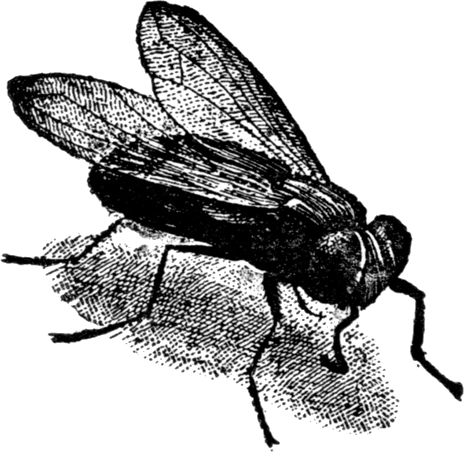
\includegraphics[height=9em]{fly.png}
\end{center}
}

\end{document}
